%! TeX program = lualatex
\documentclass[a4paper]{article} 

% packages
\usepackage{microtype}      % Slightly tweak font spacing for aesthetics
\usepackage[english]{babel} % Language hyphenation and typographical rules
\usepackage[final, colorlinks = true, urlcolor = black, linkcolor = black, citecolor = black]{hyperref} 
\usepackage{changepage}     % adjust margins on the fly
\usepackage{multicol}

\usepackage[backend=biber, style=numeric, date=iso, urldate=iso]{biblatex}
\addbibresource{references.bib}
\DeclareFieldFormat{urldate}{Accessed on: #1}

\usepackage{fontspec}
\setmainfont{EB Garamond}
\setmonofont[Scale=MatchLowercase]{Deja Vu Sans Mono}

\usepackage{minted}
\usemintedstyle{algol_nu}
\usepackage{xcolor}

\usepackage{pgfplots}
\pgfplotsset{width=\textwidth,compat=1.9}

\usepackage{caption}
\newenvironment{code}{\captionsetup{type=listing}}{}
\captionsetup[listing]{skip=0pt}
\setlength{\abovecaptionskip}{5pt}
\setlength{\belowcaptionskip}{5pt}

\usepackage[yyyymmdd]{datetime}
\renewcommand{\dateseparator}{--}

\usepackage{tikz}
\usetikzlibrary{trees}

\usepackage{titlesec}
% \titleformat{\section}{\LARGE\bfseries}{}{}{}[\titlerule]
% \titleformat{\subsection}{\Large\bfseries}{}{0em}{}
% \titlespacing{\subsection}{0em}{-0.7em}{0em}
%
% \titleformat{\subsubsection}{\large\bfseries}{}{0em}{$\bullet$ }
% \titlespacing{\subsubsection}{1em}{-0.7em}{0em}

% margins
\addtolength{\hoffset}{-2.25cm}
\addtolength{\textwidth}{4.5cm}
\addtolength{\voffset}{-3.25cm}
\addtolength{\textheight}{5cm}
\setlength{\parskip}{0pt}
\setlength{\parindent}{0in}
% \setcounter{secnumdepth}{0}

\begin{document}
\hrule \medskip
\begin{minipage}{0.295\textwidth} 
    \vfill
    \raggedright
    \footnotesize 
    \begin{tabular}{@{}l l} % Define a two-column table with left alignment
        Name: & Andrew Hayes \\
        Student ID: & 21321503 \\
        Programme: & 4BCT \\
    \end{tabular}
    \vfill
\end{minipage}
\begin{minipage}{0.4\textwidth} 
    \centering 
    \Large 
    \vfill
    \textbf{CT4101}
    \vfill
\end{minipage}
\begin{minipage}{0.295\textwidth} 
    \raggedleft
    \vfill
    \today
    \vfill
\end{minipage}
\smallskip
\hrule 
\begin{center}
    \normalsize
    Assignment 1: Classification Using Scikit-Learn
\end{center}
\hrule

% \begin{multicols}{2}
% \fontsize{9}{9}\selectfont
\section{Description of Algorithms}
\subsection{Algorithm 1: Random Forest}
% Detailed description of algorithm 1.
% Clearly describe each of your chosen scikit-learn algorithm implementations in turn, paying special attention to discussing the two hyperparameters that you have chosen to tune for each algorithm.
% You should write a maximum of 1 page per algorithm. 

\textbf{Random decision forest} is a supervised machine learning algorithm that can be used for both classification \& regression that builds upon the \textbf{decision tree} algorithm by combining several decision trees to generate labels for a dataset.
An implementation of this algorithm for classification is provided in scikit-learn as \mintinline{python}{sklearn.ensemble.RandomForestClassifier} \supercite{scikit_randomforestclassifier}.
While it can be used for regression as well as classification, I will only be referring to its use as a classification algorithm in this assignment, as regression is not relevant to the wildfire classification task at hand.
\\\\
Since the random decision forest algorithm builds upon the decision tree algorithm, it is first necessary to explain briefly what decision trees are and how they work.
A decision tree can be thought of a series of internal nodes (i.e., nodes which are not leaf nodes) that contain a question which separates the input data.
The decision tree is traversed from root to leaf for each instance being classified, where the leaf node to which we arrive is the label for that instance.
For example, a decision tree might be used to determine whether or not a living thing is a mammal, where each internal node is a question that helps to separate non-mammalian data instances from mammalian, and each leaf node is a label stating whether or not the living thing is a mammal.
Each internal node should narrow down the final label as much as possible i.e., each question should give us the maximum information about the instance and should be arranged in the order that narrows it down as quickly as possible.

\begin{figure}[H]
    \centering
    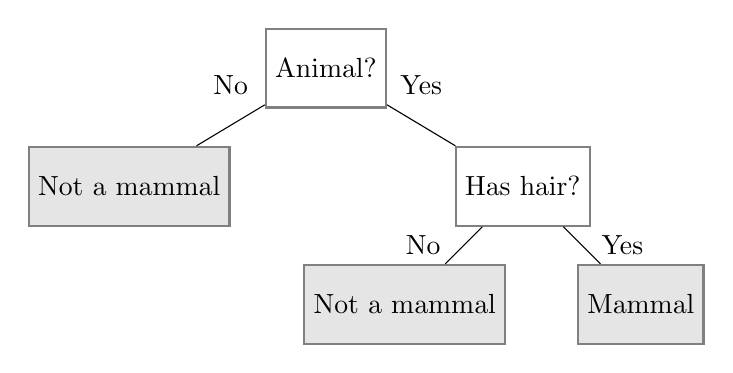
\begin{tikzpicture}[
        every node/.style={rectangle, draw=black!50, thick, minimum size=1cm},
        level 1/.style={sibling distance=5cm},
        level 2/.style={sibling distance=3cm}
    ]

    % Internal Nodes
    \node[fill=white] {Animal?}
        child { node[fill=gray!20] {Not a mammal}  edge from parent node[above, draw=none] {No} }
        child { node[fill=white] {Has hair?}
            child { node[fill=gray!20] {Not a mammal} edge from parent node[left, draw=none] {No} }
            child { node[fill=gray!20] {Mammal} edge from parent node[right, draw=none] {Yes} }
            edge from parent node[above, draw=none] {Yes}
        };

    \end{tikzpicture}
    \caption{Simplified Decision Tree to Determine Whether a Creature is a Mammal}
\end{figure}

Decision trees have many advantages: they are visualisable by humans and aren't ``black-box'', they can model non-linear relationships easily, and they are robust to outliers.
However, they have their disadvantages, including instability (small changes in the training data can significantly alter the tree structure) and in particular \textbf{overfitting}: when the algorithm fits too exactly to the training data, making it incapable of generalising to unseen data.
An extreme example of overfitting would be if the example decision tree above started to ask far too specific questions, e.g. ``Is it a dolphin'', ``Is it a human''. 
While this would have excellent performance \& accuracy on the test data, it would not work at all for an animal it hadn't encountered before.
\\\\
Random forests work by combining many decision trees into a forest, thus improving accuracy \& reducing overfitting by averaging multiple trees, reducing variance and leading to better generation.
These decision trees are each generated using random, potentially overlapping subsets of the data training data.
While the original random forest algorithm worked by taking the most popular label decided on by the set of trees \supercite{breiman}, the scikit-learn \mintinline{python}{RandomForestClassifier} works by taking a probability estimate for each label from each tree and averaging these to find the best label\supercite{scikit_ensembles}.
\\\\
In \mintinline{python}{RandomForestClassifier}, each tree is generated as follows:
\begin{enumerate}
    \item   A subset of the training data is randomly selected (hence the ``Random'' in the name of the algorithm).
            These subsets are selected ``with replacement'' which means that different trees can select the same samples: they are not removed from the pool once they are first selected.
            This results in unique, overlapping trees.
    \item   Starting with the root node, each node is \textit{split} to partition the data.
            Instead of considering all features of the samples when choosing the split, a random subset of features is selected, promoting diversity across the trees.
            The optimal split is calculated using some metric such as Gini impurity or entropy to determine which split will provide the largest reduction in impurity.
    \item   This process is repeated at every node until no further splits can be made.
\end{enumerate}

\begin{figure}[H]
\centering
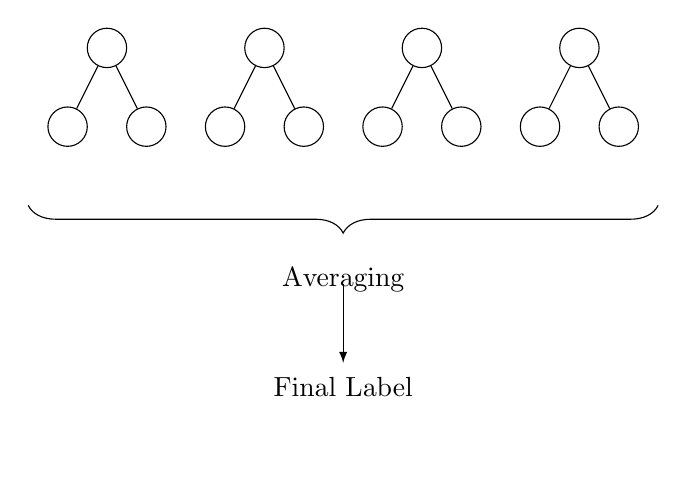
\begin{tikzpicture}[every node/.style={circle, draw, minimum size=0.5cm}]

    % Binary Trees
    \node (tree1) at (0,0) {};
    \node (tree1l) at (-0.5,-1) {};
    \node (tree1r) at (0.5,-1) {};
    \draw (tree1) -- (tree1l) {};
    \draw (tree1) -- (tree1r) {};
    
    \node (tree2) at (2,0) {};
    \node (tree2l) at (1.5,-1) {};
    \node (tree2r) at (2.5,-1) {};
    \draw (tree2) -- (tree2l) {};
    \draw (tree2) -- (tree2r) {};

    \node (tree3) at (4,0) {};
    \node (tree3l) at (3.5,-1) {};
    \node (tree3r) at (4.5,-1) {};
    \draw (tree3) -- (tree3l) {};
    \draw (tree3) -- (tree3r) {};
    
    \node (tree4) at (6,0) {};
    \node (tree4l) at (5.5,-1) {};
    \node (tree4r) at (6.5,-1) {};
    \draw (tree4) -- (tree4l) {};
    \draw (tree4) -- (tree4r) {};

    % Averaging Bracket
    \draw[decorate,decoration={brace,amplitude=10pt,mirror}] (-1,-2) -- (7,-2) node[below, midway, draw=none] {Averaging};

    % Final Label
    % \node at (4,-3) {final label};
    % \draw[->] (4,-2) -- (4,-2.5);
    \draw[-latex] (3,-3) -- (3,-4); % Adjust the coordinates as needed
    \node[draw=none] at (3,-4.3) {Final Label};
\end{tikzpicture}
\caption{Random Forest Algorithm Example Diagram (with scikit-learn Averaging)}
\end{figure}

I chose the random forest classifier because it is resistant to overfitting, works well with complex \& non-linear data like the wildfire data in question, handles both categorical \& numerical features, and offers a wide variety of hyperparameters for tuning.
It also has many benefits that are not particularly relevant to this assignment but are interesting nonetheless: it can handle both classification \& regression tasks, can handle missing data, and can be parallelised for use with large datasets.

\subsubsection{Hyperparameter 1: \mintinline{python}{n_estimators}}
The hyperparameter \mintinline{python}{n_estimators} is an \mintinline{python}{int} with a default value of 100 which controls the number of decision trees (\textit{estimators}) in the forest\supercite{scikit_randomforestclassifier}.
Increasing the number of trees in the forest typically improves the model's accuracy \& stability, with diminishing marginal returns past a certain value, at the trade-off of increased computation \& memory consumption.
Each tree is independently trained, so there is a big trade-off between computational cost \& performance.
Using a lower number of estimators can result in underfitting, as there may not be a enough trees in the forest to capture the complexity of the data.

\subsubsection{Hyperparameter 2: \mintinline{python}{max_depth}}
The hyperparameter \mintinline{python}{max_depth} is an \mintinline{python}{int} with a default value of \mintinline{python}{None} which controls the maximum ``depth'' of each of the trees in the forest \supercite{scikit_randomforestclassifier}, where the ``depth'' of a tree refers to the longest path from the root node to a leaf node in said tree.
With the default value of \mintinline{python}{None}, the trees will continue to grow until they cannot be split any further, meaning that each leaf node either only contains samples of the same class (i.e., in our case each leaf node is a definitive ``yes'' or ``no'') or contains a number of samples lower than the \mintinline{python}{min_samples_split} hyperparameter.
The \mintinline{python}{min_samples_split} hyperparameter determines the minimum number of samples required to split a node; it has a default \mintinline{python}{int} value of 2 and therefore, since I am not tuning this hyperparameter for this assignment, it has no relevance as any leaf node that doesn't reach the minimum number of samples to be split is a ``pure'' node by virtue of containing only one class.
\\\\
High \mintinline{python}{max_depth} values allow for the trees to capture more complex patterns in the data, but can overfit the data, leading to poor testing accuracy.
Bigger trees also naturally incur higher computational costs, requiring both more computation to create and more memory to store. 
Lower \mintinline{python}{max_depth} values result in simpler trees which can only focus on the most important features \& patterns in the data, which in turn can reduce overfitting;
however, low values run the risk of creating trees which are not big enough to capture the complexity of the data, and can lead to underfitting.

\subsection{Algorithm 2: C-Support Vector Classification}
\subsubsection{Hyperparameter 1: \mintinline{python}{kernel}}
\subsubsection{Hyperparameter 2: \mintinline{python}{C}}

% \section{Model Training \& Evaluation}
%
% \section{Conclusion}
%
% \bibliographystyle{plain}
% \bibliography{references}

% \end{multicols}

\nocite{*}
\printbibliography
\end{document}
